\documentclass[a4paper, 12pt]{report}
\usepackage{cmap}
\usepackage[T2A]{fontenc}
\usepackage[utf8]{inputenc}
\usepackage[english,russian]{babel}
\usepackage{listings}
\usepackage{amsmath}
\usepackage{float}
\usepackage{csquotes}
\usepackage{graphicx}
\graphicspath{ {./images/} }
\usepackage{xcolor}
\definecolor{buzzlightyear}{HTML}{8757A5}
\definecolor{grass}{HTML}{738D06}
\definecolor{literal}{HTML}{F18A2B}
\definecolor{commentcolor}{HTML}{8E908B}

\lstdefinestyle{habrstyle}{
	backgroundcolor=\color{white},
	commentstyle=\color{commentcolor},
	keywordstyle=\bfseries\color{buzzlightyear},
	numberstyle=\tiny\color{commentcolor},
	stringstyle=\color{grass},
	basicstyle=\ttfamily\footnotesize,
	breakatwhitespace=false,         
    	breaklines=true,                 
   	captionpos=b,                    
    	keepspaces=true,                 
    	numbers=left,                    
    	numbersep=7pt,                  
    	showspaces=false,                
    	showstringspaces=false,
   	showtabs=false,                  
    	tabsize=2
}

\lstset{style=habrstyle}

\author{3530901/80201, Шелаев Н. Р.}
\title{Лабораторная работа № 6. Дискретное косинусное преобразование.}
\date{\today}

\begin{document}
	\maketitle
	\tableofcontents
	\listoffigures
	\lstlistoflistings

	\chapter{Синтез}
	Сначала изучим синтез сигналов.
	\begin{lstlisting}[language=Python,caption=Первая функция для синтеза]
		from thinkdsp import CosSignal, SumSignal

		def synthesize1(amps, fs, ts):
			components = [CosSignal(freq, amp) for amp, freq in zip(amps, fs)]
			signal = SumSignal(*components)
			ys = signal.evaluate(ts)
			return ys
	\end{lstlisting}
	\begin{lstlisting}[language=Python,caption=Вторая функция для синтеза]
		def synthesize2(amps, fs, ts):
			args = np.outer(ts, fs)
			M = np.cos(PI2 * args)
			ys = np.dot(M, amps)
			return ys
	\end{lstlisting}
	\begin{lstlisting}[language=Python,caption=Сравнение этих двух функций]
		ys1 = synthesize1(amps, fs, ts)
		ys2 = synthesize2(amps, fs, ts)
		np.max(np.abs(ys1 - ys2))
	\end{lstlisting}
	Эти две функции выдают один и тот же результат.

	\chapter{Анализ}
	Теперь приступим к анализу сигналов.
	\begin{lstlisting}[language=Python,caption=Первая функция для анализа]
		def analyze1(ys, fs, ts):
			args = np.outer(ts, fs)
			M = np.cos(PI2 * args)
			amps = np.linalg.solve(M, ys)
			return amps
	\end{lstlisting}
	\begin{lstlisting}[language=Python,caption=Первая функция для тестирования]
		def test1():
			N = 4.0
			time_unit = 0.001
			ts = np.arange(N) / N * time_unit
			max_freq = N / time_unit / 2
			fs = np.arange(N) / N * max_freq
			args = np.outer(ts, fs)
			M = np.cos(PI2 * args)
			return M

		M = test1()
		M.transpose().dot(M)
	\end{lstlisting}
	\begin{lstlisting}[language=Python,caption=Вторая функция для тестирования]
		def test2():
			N = 4.0
			ts = (0.5 + np.arange(N)) / N
			fs = (0.5 + np.arange(N)) / 2
			args = np.outer(ts, fs)
			M = np.cos(PI2 * args)
			return M
    
		M = test2()
		M.transpose().dot(M)
	\end{lstlisting}
	С помощью двух тестовых функций мы посмотрели работу первой функции для анализа и пришли к выводу, что можно использовать матричное умножение. Это сильно ускорит работу функции.
	\begin{lstlisting}[language=Python,caption=Вторая функция для анализа]
		def analyze2(ys, fs, ts):
			args = np.outer(ts, fs)
			M = np.cos(PI2 * args)
			amps = M.dot(ys) / 2
			return amps
	\end{lstlisting}
	
	\chapter{Функция ДКП-IV}
	Что же это за функция?
	\begin{lstlisting}[language=Python,caption=Функция ДКП-IV]
		def dct_iv(ys, *args):
			N = len(ys)
			ts = (0.5 + np.arange(N)) / N
			fs = (0.5 + np.arange(N)) / 2
			args = np.outer(ts, fs)
			M = np.cos(PI2 * args)
			amps = np.dot(M, ys) / 2
			return amps

		def inverse_dct_iv(amps): return dct_iv(amps) * 2
	\end{lstlisting}
	Убедились, что эта функция работает правильно.

	\chapter{Класс Dct}
	Теперь изучим предоставленный нам класс \texttt{Dct}.
	\begin{lstlisting}[language=Python,caption=Применение этого класса]
		from thinkdsp import TriangleSignal

		signal = TriangleSignal(freq = 400)
		wave = signal.make_wave(duration=1.0, framerate=10000)
		dct = wave.make_dct()
		dct.plot()
	\end{lstlisting}
	\begin{figure}[H]
		\centering
		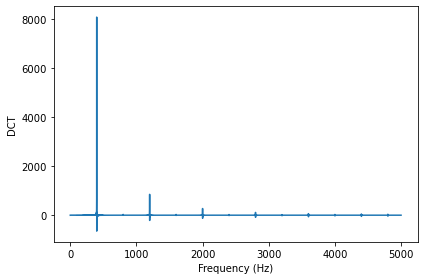
\includegraphics[width=0.75\textwidth]{dct1.png}
		\caption{Результат работы функции для тругольного сигнала}
		\label{fig:dct1}
	\end{figure}
	\begin{lstlisting}[language=Python,caption=Обратный Dct]
		signal = TriangleSignal(freq = 400, offset = 0)
		wave = signal.make_wave(duration=1.0, framerate=10000)
		wave.ys *= -1
		wave.make_dct().plot()
	\end{lstlisting}
	\begin{figure}[H]
		\centering
		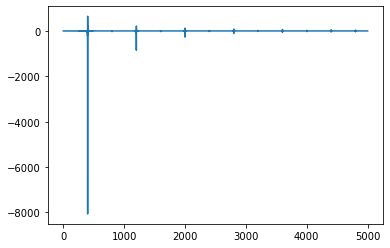
\includegraphics[width=0.75\textwidth]{dct2.png}
		\caption{Применение обратного Dct}
		\label{fig:dct2}
	\end{figure}
	
	\chapter{Упражнения}
	\section{Задание 1}
	Исследование скорости работы полученных функций.
	\begin{lstlisting}[language=Python,caption=Подготовка к исследованию]
		import scipy.fftpack		
		from scipy.stats import linregress

		signal = UncorrelatedGaussianNoise()
		noise = signal.make_wave(duration=1.0, framerate=16384)

		def scipy_dct(ys, freqs, ts): 
			return scipy.fftpack.dct(ys, type = 5)		

		def plot_bests(ns, bests):    
			plt.plot(ns, bests)
			x = np.log(ns)
			y = np.log(bests)
			t = linregress(x,y)
			slope = t[0]
			return slope

		def run_speed_test(ns, func):
			results = []
			for N in ns:
				ts = (0.5 + np.arange(N)) / N
				freqs = (0.5 + np.arange(N)) / 2
				ys = noise.ys[:N]
				result = %timeit -r1 -o func(ys, freqs, ts)
				results.append(result)    
			bests = [result.best for result in results]
			return bests
	\end{lstlisting}
	\begin{lstlisting}[language=Python,caption=Кто быстрее?]
		ns = 2 ** np.arange(6, 13)
		bests = run_speed_test(ns, analyze1)
		bests2 = run_speed_test(ns, analyze2)
		bests3 = run_speed_test(ns, scipy_dct)
		bests4 = run_speed_test(ns, dct_iv)
		plt.plot(ns, bests, label = 'analyze1')
		plt.plot(ns, bests2, label = 'analyze2')
		plt.plot(ns, bests3, label = 'fftpack.dct')
		plt.plot(ns, bests4, label = 'dct_iv')
	\end{lstlisting}
	\begin{figure}[H]
		\centering
		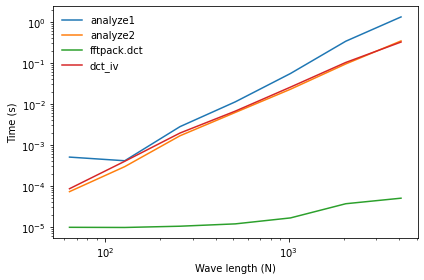
\includegraphics[width=0.75\textwidth]{dct3.png}
		\caption{Победитель очевиден}
		\label{fig:dct3}
	\end{figure}
	
	\section{Задание 2}
	Сжатие звука с помощью функции ДКП.
	\begin{lstlisting}[language=Python,caption=Получение исходного сигнала]
		from thinkdsp import read_wave

		wave = read_wave('100475__iluppai__saxophone-weep.wav')
		segment = wave.segment(start = 1.2, duration = 0.5)
		seg_dct = segment.make_dct()
		seg_dct.plot(high = 4000)
	\end{lstlisting}
	\begin{figure}[H]
		\centering
		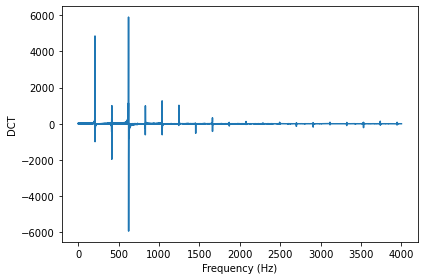
\includegraphics[width=0.75\textwidth]{dct4.png}
		\caption{До сжатия сигнала}
		\label{fig:dct4}
	\end{figure}
	\begin{lstlisting}[language=Python,caption=Функция для сжатия сигнала]
		def compress(dct, thresh = 1):
			count = 0
			for i, amp in enumerate(dct.amps):
				if np.abs(amp) < thresh:
				dct.hs[i] = 0
				count += 1       
			n = len(dct.amps)
			print(count, n, 100 * count / n, sep = '\t')

		seg_dct = segment.make_dct()
		compress(seg_dct, thresh = 10)
		seg_dct.plot(high = 4000)
	\end{lstlisting}
	\begin{figure}[H]
		\centering
		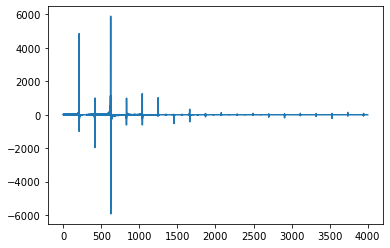
\includegraphics[width=0.75\textwidth]{dct5.png}
		\caption{После сжатия}
		\label{fig:dct5}
	\end{figure}
	\begin{lstlisting}[language=Python,caption=Применение функции для сжатия сигнала]
		from thinkdsp import Spectrogram

		def make_dct_spectrogram(wave, seg_length):
			window = np.hamming(seg_length)
			i, j = 0, seg_length
			step = seg_length // 2
			spec_map = {}
			while j < len(wave.ys):
				segment = wave.slice(i, j)
				segment.window(window)
				t = (segment.start + segment.end) / 2
				spec_map[t] = segment.make_dct()
				i += step
				j += step
			return Spectrogram(spec_map, seg_length)

		spectro = make_dct_spectrogram(wave, seg_length = 1024)

		for t, dct in sorted(spectro.spec_map.items()): compress(dct, thresh = 0.2)
	\end{lstlisting}
	Для большинства сегментов сигнала доля сжатия составила примерно 75-85\texttt{\%}. При этом звучание сигнала почти не изменилось.

	\section{Задание 3}
	Исследуем код в файле \sloppy{\texttt{phase.ipynb}}.
	\begin{lstlisting}[language=Python,caption=Начало исследования]
		from thinkdsp import SawtoothSignal

		signal = SawtoothSignal(freq = 500, offset = 0)
		wave = signal.make_wave(duration=0.5, framerate=40000)
		wave.segment(duration = 0.01).plot()
		spectrum = wave.make_spectrum()
		spectrum.plot()
	\end{lstlisting}
	\begin{figure}[H]
		\centering
		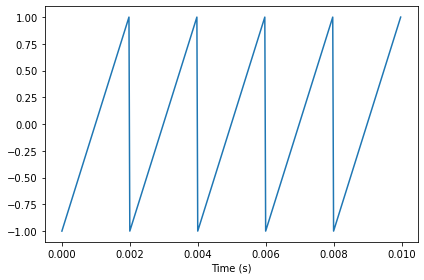
\includegraphics[width=0.75\textwidth]{test1.png}
		\caption{Сегмент пилообразного сигнала}
		\label{fig:test1}
	\end{figure}
	\begin{figure}[H]
		\centering
		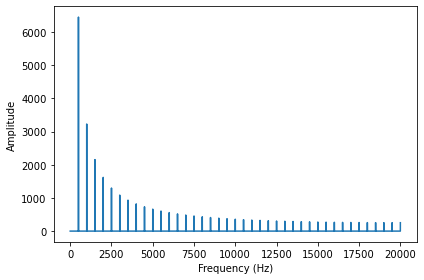
\includegraphics[width=0.75\textwidth]{test2.png}
		\caption{Спектр пилообразного сигнала}
		\label{fig:test2}
	\end{figure}
	\begin{lstlisting}[language=Python,caption=Угловая часть спектра]
		def plot_angle(spectrum, thresh = 1):
			angles = spectrum.angles
			angles[spectrum.amps < thresh] = np.nan
			plt.plot(spectrum.fs, angles, 'x')
			decorate(xlabel = 'Frequency (Hz)', ylabel = 'Phase (radian)')

		plot_angle(spectrum, thresh = 0)
		plot_angle(spectrum, thresh = 1)
	\end{lstlisting}
	\begin{figure}[H]
		\centering
		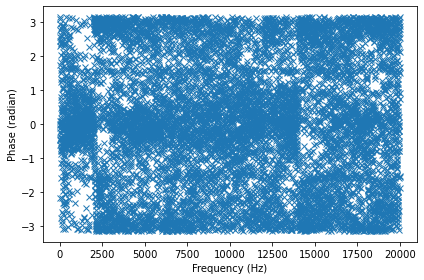
\includegraphics[width=0.75\textwidth]{test3.png}
		\caption{Все углы спектра}
		\label{fig:test3}
	\end{figure}
	\begin{figure}[H]
		\centering
		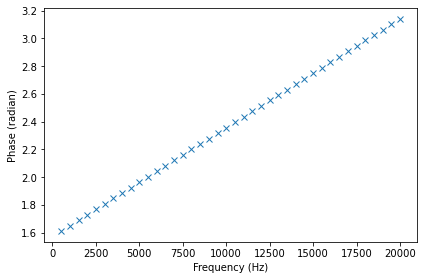
\includegraphics[width=0.75\textwidth]{test4.png}
		\caption{Структура углов}
		\label{fig:test4}
	\end{figure}
	\begin{lstlisting}[language=Python,caption=Функция для 3-х графиков]
		def plot_three(spectrum, thresh = 1):
			plt.figure(figsize = (10, 4))
			plt.subplot(1, 3, 1)
			spectrum.plot()
			plt.subplot(1, 3, 2)
			plot_angle(spectrum, thresh = thresh)
			plt.subplot(1, 3, 3)
			wave = spectrum.make_wave()
			wave.unbias()
			wave.normalize()
			wave.segment(duration = 0.01).plot()
	\end{lstlisting}
	\begin{lstlisting}[language=Python,caption=Все углы равны нулю]
		def zero_angle(spectrum):
			res = spectrum.copy()
			res.hs = res.amps
			return res
		
		spectrum2 = zero_angle(spectrum)
		plot_three(spectrum2)
	\end{lstlisting}
	\begin{figure}[H]
		\centering
		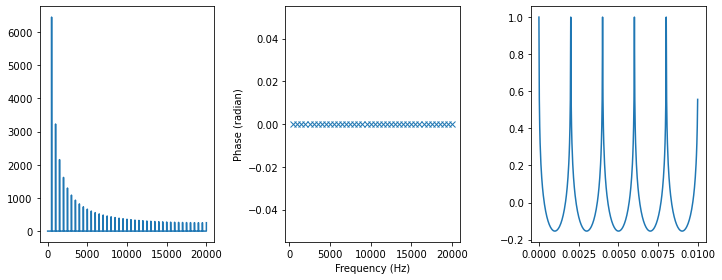
\includegraphics[width=1.0\textwidth]{test5.png}
		\caption{Нулевые углы}
		\label{fig:test5}
	\end{figure}
	\begin{lstlisting}[language=Python,caption=Функция для поворота углов]
		def rotate_angle(spectrum, offset):
			res = spectrum.copy()
			res.hs *= np.exp(1j * offset)
			return res
		
		spectrum3 = rotate_angle(spectrum, 1)
		plot_three(spectrum3)
	\end{lstlisting}
	\begin{figure}[H]
		\centering
		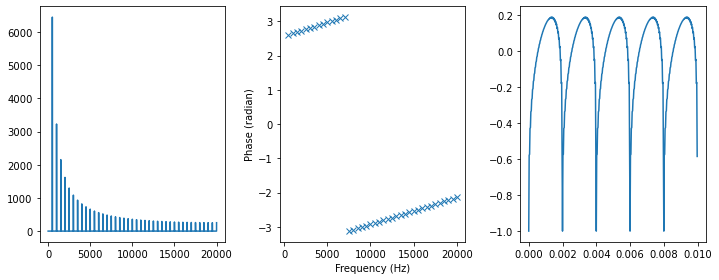
\includegraphics[width=1.0\textwidth]{test6.png}
		\caption{Результат поворота углов}
		\label{fig:test6}
	\end{figure}
	\begin{lstlisting}[language=Python,caption=Функция для генерации случайных углов]
		def random_angle(spectrum):
			res = spectrum.copy()
			angles = np.random.uniform(0, PI2, len(spectrum))
			res.hs *= np.exp(1j * angles)
			return res

		spectrum4 = random_angle(spectrum)
		plot_three(spectrum4)
	\end{lstlisting}
	\begin{figure}[H]
		\centering
		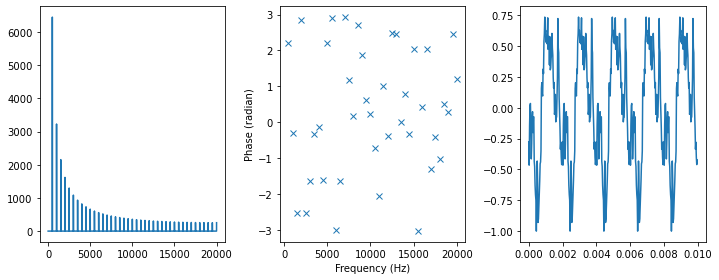
\includegraphics[width=1.0\textwidth]{test7.png}
		\caption{Слачайные углы}
		\label{fig:test7}
	\end{figure}
	\begin{lstlisting}[language=Python,caption=Исходный сигнал]
		from thinkdsp import read_wave

		wave = read_wave('120994__thirsk__120-oboe.wav')
		segment = wave.segment(start = 0.05, duration = 0.9)
		spectrum = segment.make_spectrum()
		plot_three(spectrum, thresh = 50)
	\end{lstlisting}
	\begin{figure}[H]
		\centering
		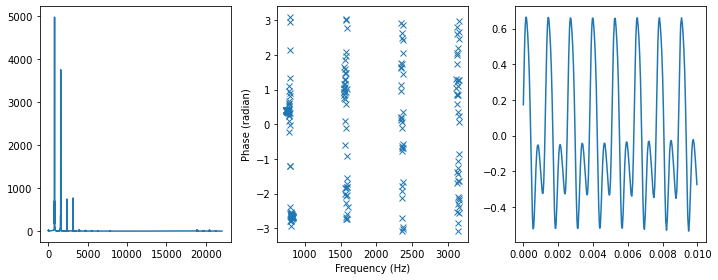
\includegraphics[width=1.0\textwidth]{test8.png}
		\caption{Исходный сегмент}
		\label{fig:test8}
	\end{figure}
	\begin{lstlisting}[language=Python,caption=Применение функций]
		spectrum2 = zero_angle(spectrum)
		plot_three(spectrum2, thresh = 50)
		
		spectrum3 = rotate_angle(spectrum, 1)
		plot_three(spectrum3, thresh = 50)

		spectrum4 = random_angle(spectrum)
		plot_three(spectrum4, thresh = 50)
	\end{lstlisting}
	\begin{figure}[H]
		\centering
		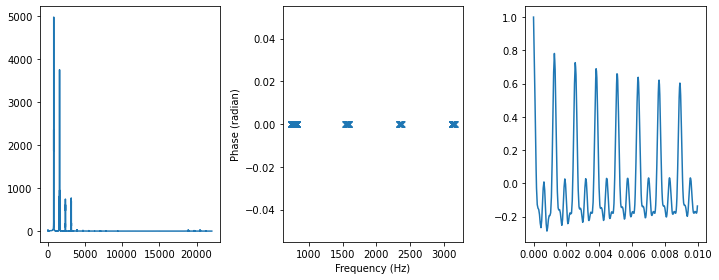
\includegraphics[width=1.0\textwidth]{test9.png}
		\caption{Занулили углы}
		\label{fig:test9}
	\end{figure}
	\begin{figure}[H]
		\centering
		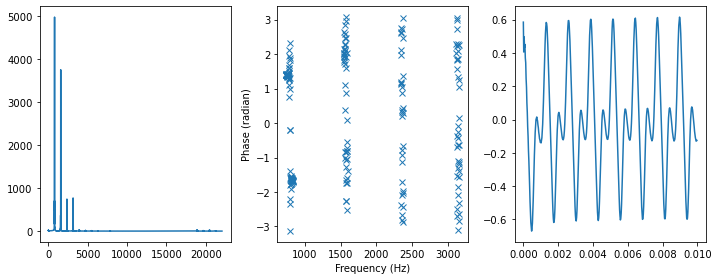
\includegraphics[width=1.0\textwidth]{test10.png}
		\caption{Повернули}
		\label{fig:test10}
	\end{figure}
	\begin{figure}[H]
		\centering
		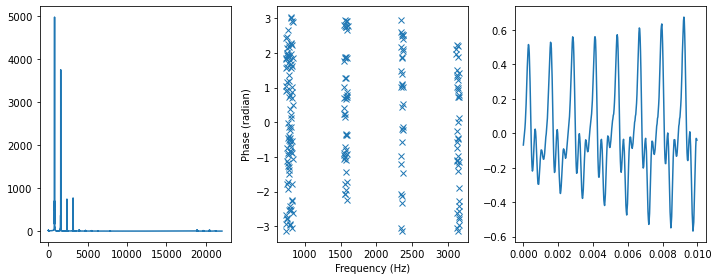
\includegraphics[width=1.0\textwidth]{test11.png}
		\caption{Случайные значения}
		\label{fig:test11}
	\end{figure}
	\begin{lstlisting}[language=Python,caption=Возьмём другой сигнал]
		wave = read_wave('100475__iluppai__saxophone-weep.wav')
		wave.make_audio()
		segment = wave.segment(start = 1.9, duration = 0.6)
		spectrum = segment.make_spectrum()
		plot_three(spectrum, thresh = 50)
	\end{lstlisting}
	\begin{figure}[H]
		\centering
		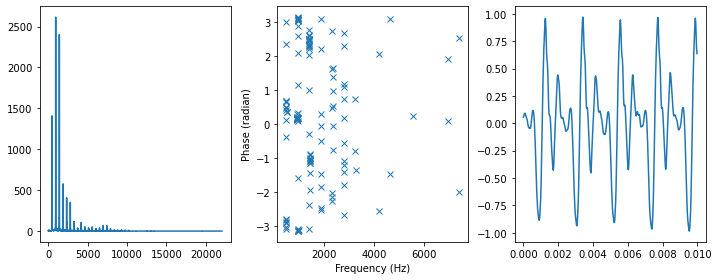
\includegraphics[width=1.0\textwidth]{test12.png}
		\caption{Исходный сигнал}
		\label{fig:test12}
	\end{figure}
	\begin{lstlisting}[language=Python,caption=Применение функций для другого сигнала]
		spectrum2 = zero_angle(spectrum)
		plot_three(spectrum2, thresh = 50)
		...
	\end{lstlisting}
	\begin{figure}[H]
		\centering
		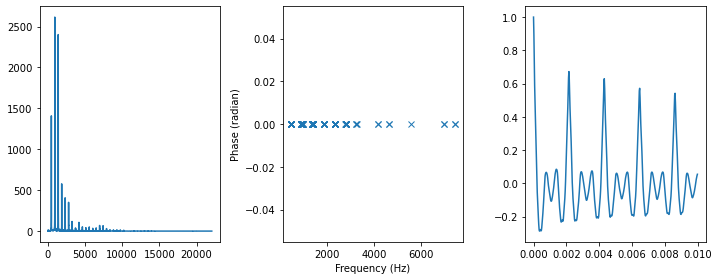
\includegraphics[width=1.0\textwidth]{test13.png}
		\caption{Углы = 0}
		\label{fig:test13}
	\end{figure}
	\begin{figure}[H]
		\centering
		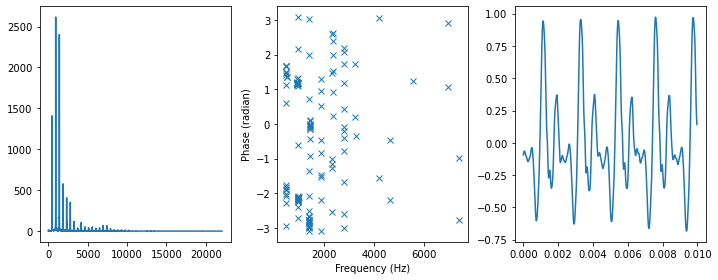
\includegraphics[width=1.0\textwidth]{test14.png}
		\caption{Поворот углов на 1 радиан}
		\label{fig:test14}
	\end{figure}
	\begin{figure}[H]
		\centering
		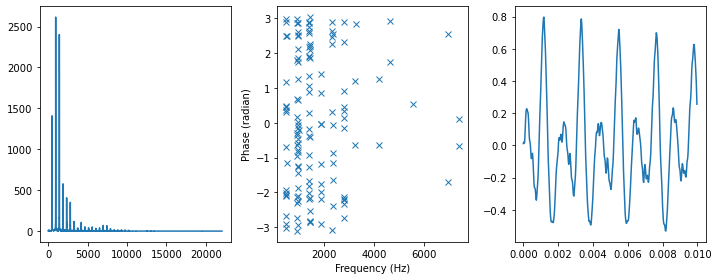
\includegraphics[width=1.0\textwidth]{test15.png}
		\caption{Random}
		\label{fig:test15}
	\end{figure}
	\begin{lstlisting}[language=Python,caption=Применили ФВЧ для сигнала]
		spectrum.high_pass(600)
		spectrum.plot(high = 4000)
		plot_three(spectrum2, thresh = 50)
	\end{lstlisting}
	\begin{figure}[H]
		\centering
		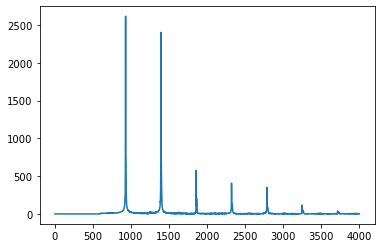
\includegraphics[width=0.75\textwidth]{test16.png}
		\caption{Спектр сигнала изменился}
		\label{fig:test16}
	\end{figure}
	\begin{figure}[H]
		\centering
		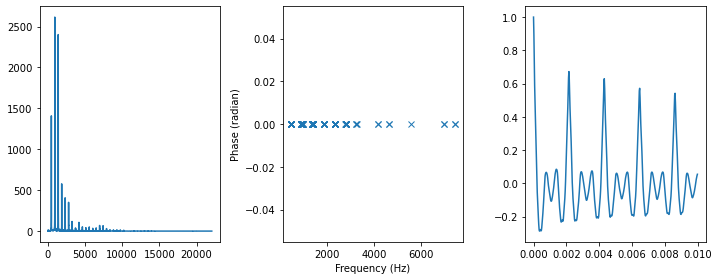
\includegraphics[width=1.0\textwidth]{test17.png}
		\caption{Исходный сигнал после ФВЧ}
		\label{fig:test17}
	\end{figure}
	\begin{lstlisting}[language=Python,caption=Применение функций сигнала после ФВЧ]
		spectrum2 = zero_angle(spectrum)
		plot_three(spectrum2, thresh = 50)
		...
	\end{lstlisting}
	\begin{figure}[H]
		\centering
		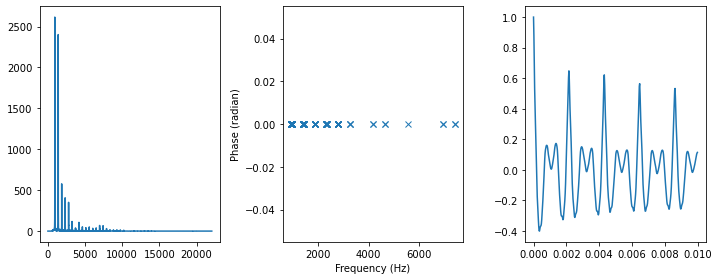
\includegraphics[width=1.0\textwidth]{test18.png}
		\caption{Обнуление углов}
		\label{fig:test18}
	\end{figure}
	\begin{figure}[H]
		\centering
		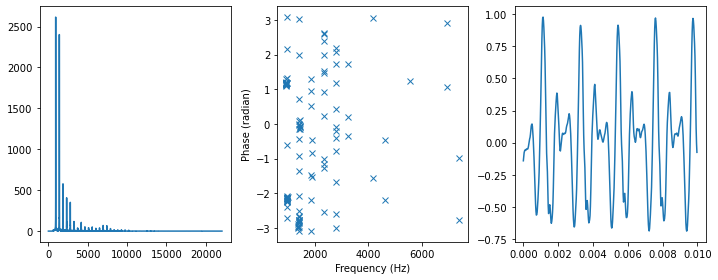
\includegraphics[width=1.0\textwidth]{test19.png}
		\caption{1 радиан}
		\label{fig:test19}
	\end{figure}
	\begin{figure}[H]
		\centering
		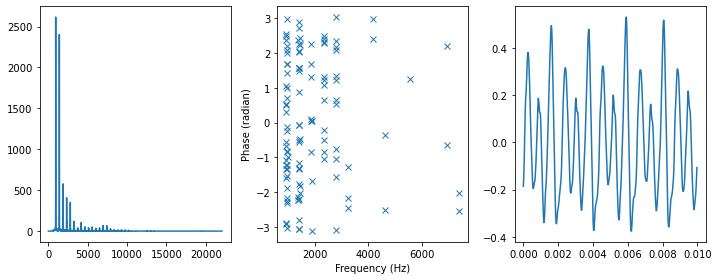
\includegraphics[width=1.0\textwidth]{test20.png}
		\caption{Случайность}
		\label{fig:test20}
	\end{figure}
	Мы не услышали каких-либо изменений в сигналах.

	\chapter{Вывод}
	В данной работе мы изучили и применили различные функции для анализа и синтеза сигналов. Встроенная функция \texttt{Dct} для анализа оказалась быстрее других алгоритмов.Также применили функции ДКП для сжатия сигналов.
\end{document}